%%%%%%%%%%%%%%%%%%%%%%%%%%%%%%%%%%%%%%%%%%%%%%%%%%%%%%%%%%%%%%%%%%%%%
%
% VC36O Writeup Template
%
% This is a LaTeX document. LaTeX is a markup language for producing 
% documents. Your task is to fill out this
% document, then to compile this into a PDF document. 
% You will then upload this PDF to `Moodle'.
%
% 
% TO COMPILE:
% > pdflatex thisfile.tex
%
% For references to appear correctly instead of as '??', you must run 
% pdflatex twice.
%
% If you do not have LaTeX and need a LaTeX distribution:
% - Personal laptops (all common OS): www.latex-project.org/get/
%
% If you need help with LaTeX, please come to office hours. 
% Or, there is plenty of help online:
% https://en.wikibooks.org/wiki/LaTeX
%
% Good luck!
%
%%%%%%%%%%%%%%%%%%%%%%%%%%%%%%%%%%%%%%%%%%%%%%%%%%%%%%%%%%%%%%%%%%%%%
%
% How to include two graphics on the same line:
% 
% \includegraphics[\width=0.49\linewidth]{yourgraphic1.png}
% \includegraphics[\width=0.49\linewidth]{yourgraphic2.png}
%
% How to include equations:
%
% \begin{equation}
% y = mx+c
% \end{equation}
% 
%%%%%%%%%%%%%%%%%%%%%%%%%%%%%%%%%%%%%%%%%%%%%%%%%%%%%%%%%%%%%%%%%%%%%%%%%%%%%%%%%%%%%%%%%%%%%%%%

\documentclass[11pt]{article}

\usepackage[english]{babel}
\usepackage[utf8]{inputenc}
\usepackage[colorlinks = true,
            linkcolor = blue,
            urlcolor  = blue]{hyperref}
\usepackage[a4paper,margin=1.5in]{geometry}
\usepackage{stackengine,graphicx}
\usepackage{fancyhdr}
\setlength{\headheight}{15pt}
\usepackage{microtype}
\usepackage{times}
\usepackage{booktabs}

% From https://ctan.org/pkg/matlab-prettifier
\usepackage[numbered,framed]{matlab-prettifier}

\frenchspacing
\setlength{\parindent}{0cm} % Default is 15pt.
\setlength{\parskip}{0.3cm plus1mm minus1mm}

\pagestyle{fancy}
\fancyhf{}
\lhead{Project Writeup}
\rhead{VC36O 2018/1}
\rfoot{\thepage}

\date{}

\title{\vspace{-1cm}Project 4 Writeup}


\begin{document}
\maketitle
\vspace{-3cm}
\thispagestyle{fancy}

%\section*{Instructions}
%\begin{itemize}
%  \item Describe any interesting decisions you made to write your algorithm.
%  \item Show and discuss the results of your algorithm.
%  \item Feel free to include code snippets, images, and equations.
%  \item Use as many pages as you need, but err on the short side If you feel you only need to write a short amount to meet the brief, th
  
%  \item \textbf{Please make this document anonymous.}
%\end{itemize}

\section*{In the beginning...}

A calibração de câmera geométrica, também conhecida como ressecção de câmera, determina os parâmetros de uma lente e sensor de imagem de uma câmera de vídeo ou foto. Pode-se utilizar esses parâmetros para corrigir a distorção da lente, medir o tamanho de um objeto ou determinar a localização da câmera na cena (Figura~\ref{fig:1}). Esses métodos são usados em aplicativos como visão de máquina para detectar e medir objetos, robótica, sistemas de navegação e reconstrução de cenas tridimensionais \cite{Matlab}.

Os parâmetros da câmera incluem coeficientes intrínsecos, extrínsecos e de distorção. Para estimar esses parâmetros, é necessários de pontos 3D e 2D de imagens correspondentes. Tais correspondências podem ser obtidas utilizando diversas imagens de um padrão de calibração, como um tabuleiro de damas. Com as correspondências, é possível resolver os parâmetros da câmera. Depois de calibrar uma câmera, para avaliar a precisão dos parâmetros estimados, é possível plotar as localizações relativas da câmera e o padrão de calibração, calcular os erros de reprojeção e os erros de estimativa de parâmetros.\cite{Matlab}:



\begin{figure}[h]
    \centering
    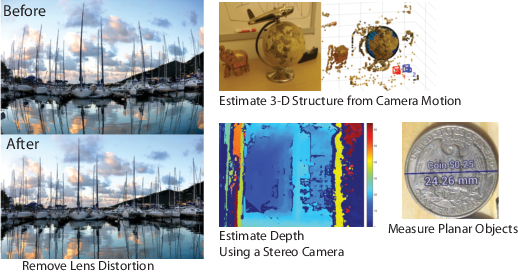
\includegraphics[width=8cm]{calibration_applications.png}
    \caption{Aplicações da calibração de câmera geométrica.}
    \label{fig:1}
\end{figure}

O consenso de amostra aleatória (RANSAC), é um método iterativo para estimar um modelo matemático de um conjunto de dados que contém \textit{outliers}. O algoritmo RANSAC funciona identificando os outliers em um conjunto de dados e estimando o modelo desejado usando dados que não contêm \textit{outliers}\cite{Ransac}.

Primeiramente o código do RANSAC seleciona aleatoriamente um subconjunto do conjunto de dados; depois ajusta um modelo ao subconjunto selecionado; determina o número de \textit{outliers}; e por fim, repete os passos anteriores para um número determinado de iterações \cite{Ransac}.

Na visão computacional, o RANSAC é usado como uma abordagem robusta para estimar a matriz fundamental em visão estéreo, para encontrar a semelhança entre dois conjuntos de pontos para detecção de objetos baseada em recursos e registrar quadros de vídeo sequenciais para estabilização de vídeo \cite{Ransac}.

O objetivo deste trabalho é apresentar a câmera e a geometria da cena, estimando a matriz de projeção da câmera, que mapeia coordenadas do mundo 3D para as coordenadas da imagem, bem como a matriz fundamental, que relaciona pontos em uma cena a linhas epipolares em outra. A matriz de projeção da câmera e a matriz fundamental podem ser estimadas usando correspondências pontuais. Para determinar a matriz fundamental, a entrada corresponde a 2D pontos em duas imagens. A matriz fundamental pode ser estimada usando as correspondências pontuais de RANSAC \cite{Trab}.


\section*{Interesting Implementation Detail}
Este trabalho possui três partes:
\begin{enumerate}
\item Estimar a matriz de projeção;
\item Estimar a matriz fundamental;
\item Estimar a matriz fundamental de forma confiável com o RANSAC a partir de correspondências não confiáveis do SIFT.

\end{enumerate}

As partes 1 e 2 já foram disponibilizada prontas, sendo necessário apenas criar a parte 3, que foi implementada no código \texttt{ransac\_fundamental\_matrix.m}. Basicamente, o algoritmo deve estimar uma matriz fundamental baseada na escolha de 8 pontos aleatórios de um conjunto de pontos pertencentes a duas imagens. Essa matriz é utilizada para definir \textit{inliers}  que melhoram a precisão de correspondências obtidas pelo algoritmo do SIFT. 

Inicialmente, foi definido o número de interações em que o algoritmo deve ser executado, que depende de um número de pontos (linha 1), um limite de erro (linha 2), uma taxa de confiança (linha 3) e uma função utilizando log (linha 4), como descrito a seguir:

\begin{lstlisting}[style=Matlab-editor]
pontPorInter = 8; %quantidade de pontos
distThresold = 0.05; %limite aceitavel de erro 
p = 0.99; % taxa confianca
N = log(1-p)/log(1-(1-distThresold).^pontPorInter);
\end{lstlisting}

Dentro do laço de repetição, por meio da função \texttt{randi}, foi definido os 8 pontos aleatórios de cada conjunto de pontos das imagens (\textit{matches\_a} e \textit{matches\_b}) (linhas 4, 5 e 6). Com esses pontos foi possível obter a matriz fundamental utilizando uma função denominada \texttt{estimate\_fundamental\_matrix}(linha 9), como demonstra o código a seguir:

\begin{lstlisting}[style=Matlab-editor]
(...)
for i=1: N
  % Escolher aleatoriamente 8 pontos de cada matches
  ponts = randi(size(matches_a,1), [pontPorInter,1]);
  ponts_match_a = matches_a(ponts,:);
  ponts_match_b = matches_b(ponts,:);

  %Obter a matriz fundamental
  Fmatrix = estimate_fundamental_matrix(ponts_match_a, ponts_match_b)
(...)
\end{lstlisting}

Sabendo a matriz fundamental, foi necessário definir uma métrica capaz de encontrar os \textit{inliers} do conjunto de pontos das imagens (\textit{matches\_a} e \textit{matches\_b}). Essa métrica, consistiu em um somatório que multiplica \texttt{xb}, matriz fundamental e \texttt{xa'}, onde \texttt{xb} e \texttt{xa} são, respectivamente, os \textit{matches} b e a com uma dimensão a mais contendo apenas o valor 1. As linhas 4, 5, 7, 8, 10 e 11 do código a seguir demonstra como foi obtido as matrizes \texttt{xa} e \texttt{xb}. Já a linha 15 demonstra a métrica utilizada:

\begin{lstlisting}[style=Matlab-editor]
(...)

% defirnir matriz auxiliar para utilizar na metrica de distancia
tamMatches_a = size(matches_a, 1); %tamanho da matriz mataches_a
tamMatches_b = size(matches_b,1); % tamanho da matriz matches_b
%criar um vetor de 1 com tamanho dos matches_a e b
one_matches_a = ones(tamMatches_a,1);
one_matches_b = ones(tamMatches_b,1);
%criar matriz igual a matches_a e b com uma coluna a mais contendo valores 1
xa = [matches_a one_matches_a];
xb = [matches_b one_matches_b];

(...)
%calcular metrica de distancia baseada na matriz fundamental para contar o numero de inliers (xb * F * xa')
metrica = sum((xb .* (Fmatrix * xa')'),2); % xb * F * xa'

(...)  
\end{lstlisting}

Com a métrica, foi possível determinar o vetor de \textit{inliers} considerando um limite de erro pré-definido, e a sua quantidade. A linha 3 a seguir demonstra como foi determinado esse vetor, e a linha 5 como foi definido o tamanho dos \textit{inliers}:  

\begin{lstlisting}[style=Matlab-editor]
(...)
 %vetor de inliers
  limEr = find(abs(metrica) <= distThresold); 
  % encontra o numero de inliers
  inliers = size( limEr , 1);  
  (...)  
\end{lstlisting}

A cada interação do algoritmo, foi armazenada a matriz fundamental e o vetor que apresentou o maior número de \textit{inliers}. Para isso, foi feito uma comparação simples, como demonstra a condição das linhas 2 a 6 a seguir:

\begin{lstlisting}[style=Matlab-editor]
(...)
 if (inliers > maxInliers)
     Best_Fmatrix = Fmatrix;
     maxInliers = inliers
     %armazenar o vetor de inliers correpondete ao maxInliers
     currentInliers  = limEr;   
  end 
  (...)  
\end{lstlisting}

Ao final, foi retornado na função os \textit{inliers} encontrados correspondentes aos \textit{matches} a e b. Para isso, foi armazenado os \textit{matches} nas posições dos \textit{inliers} encontrados, e a quantidade desses \textit{matches} equivale ao número máximo de \textit{inliers} encontrado, como mostra a linha 3 e 4 a seguir:

\begin{lstlisting}[style=Matlab-editor]
(...)
%encontrar os inliers a e b de acordo com o maximo inliers encontrado
inliers_a = matches_a(currentInliers(1:maxInliers),:);
inliers_b = matches_b(currentInliers(1:maxInliers),:);
(...)  
\end{lstlisting}

\section*{A Result}

O primeiro resultado foi satisfatório, pois as correspondências obtidas utilizando o RANSAC implementado foram melhores do que utilizando apenas o SIFT. A Figura~\ref{fig:sift} mostra o resultado da imagem Mount Rushmore utilizando apenas o SIFIT. Já a Figura~\ref{fig:rasac1} apresenta a mesma imagem, porém utilizando o RANSAC.


\begin{figure}[h]
    \centering
    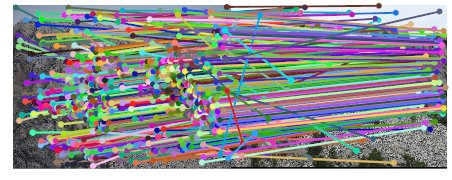
\includegraphics[width=8cm]{sift.jpg}
    \caption{Correspondências Mount Rushmore utilizando SIFIT.}
    \label{fig:sift}
\end{figure}

\begin{figure}[h]
    \centering
    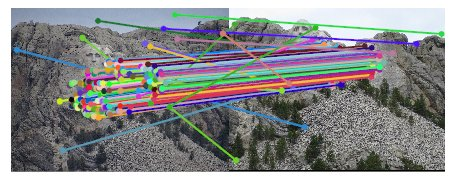
\includegraphics[width=8cm]{ransac1.jpg}
    \caption{Correspondências Mount Rushmore utilizando RANSAC implementado.}
    \label{fig:rasac1}
\end{figure}


É possível observar que o uso do RANSAC melhora várias correspondências erradas do SIFIT, entretanto piora outras. Para aprimorar esse resultado, foi re-estimada a matriz fundamental usando todos os \textit{inliers} encontrados pelo RANSAC. A Figura~\ref{fig:rasac2} mostra o resultado obtido.

\begin{figure}[h]
    \centering
    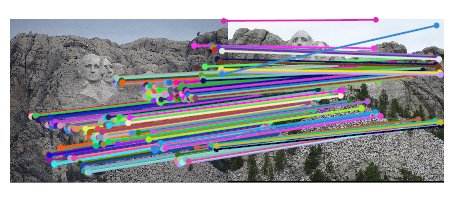
\includegraphics[width=8cm]{ransac2.jpg}
    \caption{Correspondências Mount Rushmore obtida pela re-estimação da matriz fundamental usando todos os inliers.}
    \label{fig:rasac2}
\end{figure}

É possível observar que os resultados após a re-estimação da matriz fundamental foi extremamente satisfatório, pois quase todas as correspondências foram estimadas de forma correta.


\bibliographystyle{abntex2-alf}
\bibliography{references}


\end{document}
